\section{General description}

\subsection{Product perspective}
 %Describes the environment of the system

\subsubsection{Description}
This is a new product which will be able to work together with other messaging capabilities, such as normal messaging on mobile devices, and also other applications capable of using the basic GSM character set.
\vspace{12pt}\\
GSM character set only allows a number of characters which may prevent the use of certain encryption. Many encryption algorithms greatly increase the number of characters, but this approach will be infeasable.
\vspace{12pt}\\
Software interface - The software interface will make use of the clipboard functionality on the phone in order to copy and paste messages or ciphertexts.
\vspace{12pt}\\
User interface - The user interface is what will allow the user to encrypt a message and decrypt a message which has been sent by other users of this application.
\vspace{12pt}\\
Hardware Interface - The software will run on a mobile device with touch screen capabilities.


%Note:
%Required : Functionality must be provided if service is provided
%Extends : Extended functionality which can be provided, but not always.
\newpage
\subsubsection{Use Cases}
SMSEncryption Use case diagram

\begin{center}
 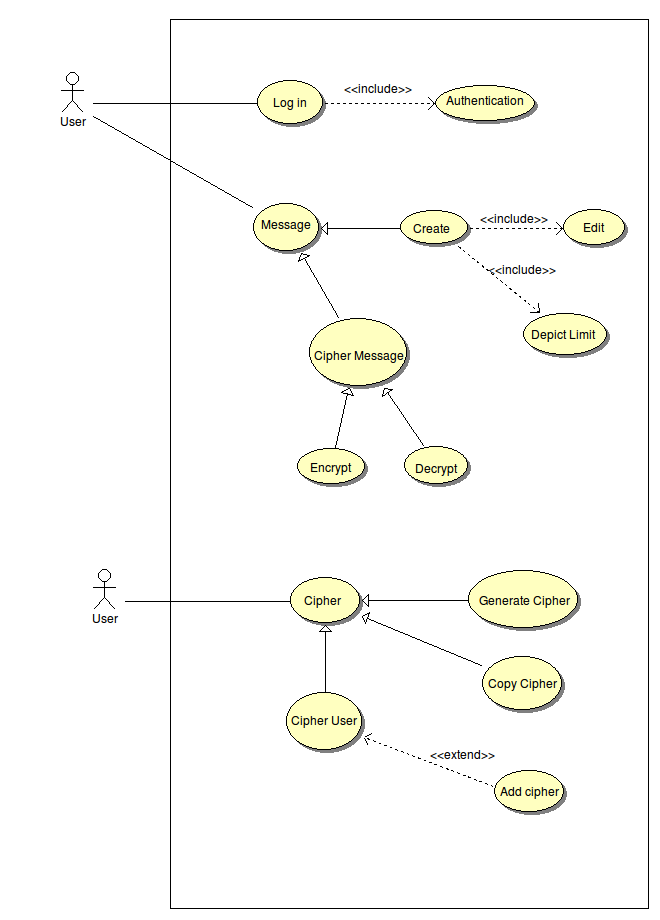
\includegraphics[width=13cm]{diagrams/UseCaseDiagrams/UseCaseSMSEncryption.png}
\end{center}




\subsection{Product features}
%An overview of the system's main features
%? complete list of "brief" use-case descriptions
%? features will be specified in detail in Section 3
\subsubsection{Log In}
\begin{itemize}
\item The application will ask the user for login details which he/she must then enter in correctly. 
\item If it is incorrect, the application will close preventing access for an unauthorised user.
\end{itemize}
\subsubsection{Message}
\textbf{Create}
\begin{itemize}
\item The user can create a message using this application.
\item The application will also allow the user to edit the message which is currently being typed in.
\item The limit of the message will be displayed while the user is entering a message.
\end{itemize}
\textbf{Cipher Message}
\begin{itemize}
\item The message can be encrypted to obtain the cipher text which the user can send to the other user. 
\item The cipher text can be sent after copying the message to the clipboard and pasting it into a message such as SMS or other similar applications.
\item The user who receives a message will be able to decrypt the message afterwards showing the original message before encryption.
\end{itemize}


\subsubsection{Cipher}
\begin{itemize}
\item The user can generate a cipher which will influence how it is encrypted and decrypted by the sender and receiver. 
\item This cypher can be copied and can be used in other places such as add cipher.
\item The user can add a cipher to the application determining how the message will be encrypted and decrypted which allows communication between two users.
\end{itemize}

\subsection{User characteristics}
%Assumptions about the users, their background, how
%much training they will need
%? e.g., different user interfaces for expert vs. novice users
%? Only user characteristics that affect the software
%requirements
\begin{itemize}
\item There will be only one user class who will have full access to all the features provided by the application.
\item It is assumed that the user has proficient knowledge on how to copy items from messages such as SMS and paste it within this application.
\end{itemize}


\subsection{Constraints}
%Anything that will limit the designer's options
\begin{itemize}
\item The application must make use of the basic GSM character set.
\item The application will be delivered as a prototype if time permits.
\end{itemize}



\subsection{Assumptions and dependencies}
%List any assumed factors (as opposed to known facts) 
%that could affect the requirements stated in the SRS. 

\begin{itemize}
\item It is assumed that the amount of characters in the basic GSM character set is 128 for the 7-bit encoding used in GSM.
\end{itemize}
